\subsection{Fixed load sampling}
\subsubsection{Problem Statement}
We suppose that sometimes learning can happen in unrealistic and undesirable ways. 
Consider a controller that simply raises the prices arbitrarily, or reduces prices arbitrarily. 
We propose that the samples of prices should be with respect to a constant load of magnitude $ c$. 
This way the price vector across the the day is equal to 
\begin{align*}
  P &= c p_1 + c p_2 + \ldots c p_{10} \\
    &= c(p_1 + p_2 + \ldots p_{10}) \\
    &= c \lVert \vec{p} \rVert_1
\end{align*}
So the magnitude is constant. 
\subsubsection{L1 Norm}
We observe that now our problem is equivalent to sampling $ \vec{p}$ with a fixed L1 norm. 

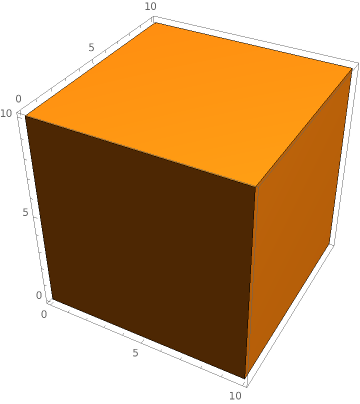
\includegraphics[width=2cm]{graphics/box_uniform.png} $\rightarrow$  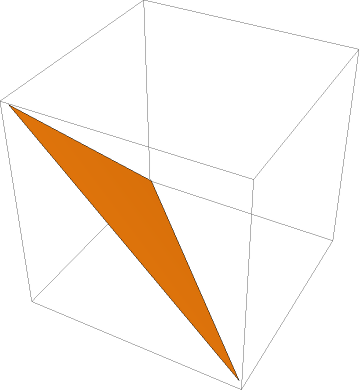
\includegraphics[width=2cm]{graphics/tri_uniform.png}
    
    
\red{Will idk what you want to add here. Sorry for the late addition.}
